\chapter{Methodik}
\label{ch:methods}

\lstdefinelanguage{json}{
    breaklines=true,
}

\begin{figure}[tb]
    \centering
    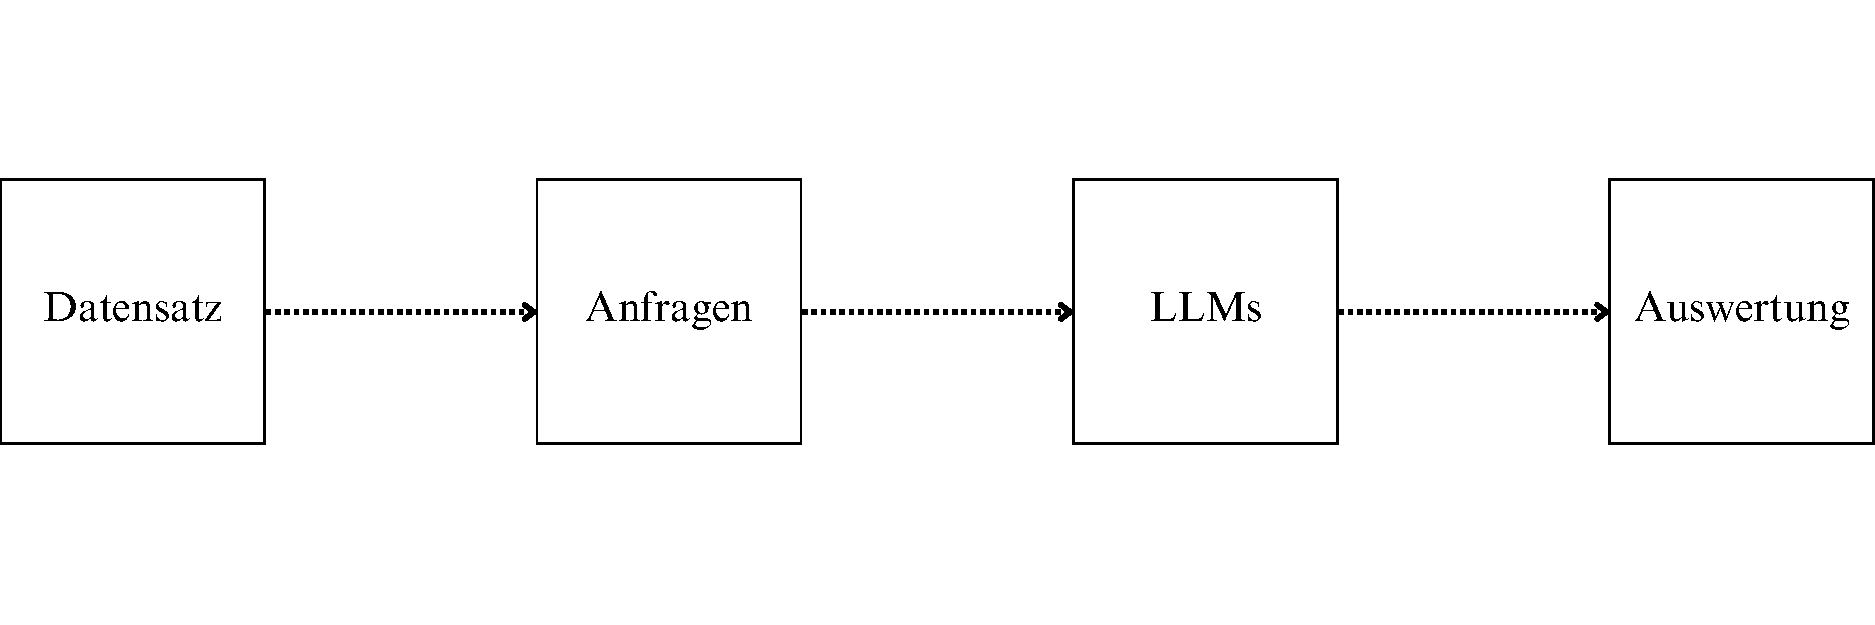
\includegraphics[width=0.95\columnwidth]{img/Ablaufdiagramm.pdf}%
    \caption{Grundstruktur der Experimente.}
    \label{fig_ablauf}
\end{figure}

Zur Beantwortung der Fragestellung werden zwei Experimente durchgeführt.
Im ersten Experiment werden verschiedene Llama 3 Modelle nach den Koordinaten bestimmter Städte befragt.
Die auf diese Weise erhaltenen Antworten werden anschließend mit den tatsächlichen Werten verglichen.
Im zweiten Experiment soll die Distanz zwischen zwei Städten bestimmt werden. Auch diese wird mit der tatsächlichen Distanz verglichen.

Beide Experimente folgen der in Abbildung \ref{fig_ablauf} dargestellten Grundstruktur. Zunächst wird ein passender Datensatz erstellt und daraus entsprechende Anfragen generiert. Diese Anfragen werden an verschiedene LLMs gestellt und die Antworten anschließend für die Analyse aufbereitet, die in Kapitel \ref{ch:results} vorgestellt wird.

Die praktische Umsetzung der Methodik, die gesammelten Daten und die Auswertungen sind zu finden unter: \url{https://github.com/JustusKlameth/ba-dev}.

\section{Koordinaten}
\label{methods_coords}
In diesem Experiment wird der Fokus darauf gelegt zu ermitteln, \textit{in welchem Umfang ausgewählte Llama 3 Modelle in der Lage sind, akkurate Koordinaten für Städte anzugeben}.
Zu diesem Zweck werden die Llama 3 Modelle ähnlich zur Vorgehensweise von \mbox{\citet{bhandariAreLargeLanguage2023}} nach den Koordinaten von Städten befragt und die daraus resultierenden Antworten ausgewertet.

Darüber hinaus werden drei verschiedene Methoden getestet, um die angestrebten Informationen zu erlangen.
Des Weiteren wird untersucht, welchen Einfluss es hat, zusätzlich zum Städtenamen auch das zugehörige Land zu übergeben.

\subsection{Datensatz}
\label{ss:methods:coords:data}
Der Datensatz umfasst die global verteilten 3.527 Städte aus dem MaxMind Datensatz\footnote{\url{https://www.kaggle.com/datasets/max-mind/world-cities-database}} mit mindestens 100.000 Einwohnern.
Dieser Datensatz wurde ausgewählt, weil er alle für die Auswertung relevanten Informationen enthält (Städtename, Ländercode, Längen- und Breitengrad).
Außerdem erlaubt dieser Datensatz einen Vergleich mit den Ergebnissen von \citet{bhandariAreLargeLanguage2023}.

\subsection{Anfragen}
Die Generierung von Anfragen erfolgt unter Anwendung der Vorlagen \ref{fig_template_json} und \ref{fig_template_original}, wobei für \textit{\{location\}} der Städtename eingesetzt wird.
Darüber hinaus besteht die Option, neben dem Städtenamen auch das zugehörige Land zu verwenden.

Für jede Stadt in dem Datensatz werden vier Anfragen erstellt, also für jede Vorlage einmal mit und einmal ohne die Länderinformation.

Die Vorlage \ref{fig_template_original} wurde ausgewählt, da \citet{bhandariAreLargeLanguage2023} auf diese Weise bereits vielversprechende Ergebnisse mit älteren Llama Modellen erzielt haben.
Zusätzlich wurde die Vorlage \ref{fig_template_json} als Kontrast entwickelt, da sie weniger allgemeine Vorgaben enthält, dafür aber ein festes Antwortformat vorschreibt und damit einen neuen Ansatz verfolgt.

\begin{figure}[tb] % json-Vorlage
    \lstinputlisting[language=json]{code/json.json}
    \caption{Diese Vorlage schreibt das \textit{json}-Format für die Antwort vor. Dafür wird nicht explizit (wie bei \ref{fig_template_original}) darauf hingewiesen, keine falschen Informationen zu verbreiten.}
    \label{fig_template_json}
\end{figure}

\begin{figure}[tb] % originale-Vorlage
    \lstinputlisting[language=json]{code/original.json}
    \caption{Vorlage von \citet{bhandariAreLargeLanguage2023}. Diese Vorlage nutzt eine offene Formulierung und schreibt kein Antwortformat vor.}
    \label{fig_template_original}
\end{figure}

\subsection{LLMs}
Mit diesen Anfragen werden das Llama-3.3-70B-Instruct Modell und die Llama-3.1-Instruct Modelle in den Größen 8B, 70B und 405B getestet.
Dafür wird DeepInfra\footnote{\url{https://deepinfra.com/}} genutzt.

Die Llama 3.1 Modelle wurden ausgewählt, da sie die größte Spanne an Parametergrößen innerhalb einer Version liefern und somit einen umfassenden Vergleich ermöglichen.
Das Llama 3.3 Modell wurde zusätzlich betrachtet, um festzustellen, ob es bei gleicher Parameteranzahl eine Verbesserung des geographischen Wissens gibt.

\subsection{Auswertung}
\label{ss:methods:coords:verfahren}
Um die Qualität der Antworten messen zu können, wird als Fehler die geodätische Distanz zwischen den tatsächlichen Koordinaten der Stadt und den Koordinaten der Antwort des LLMs verwendet.
Dafür wird der Algorithmus von \citet{karneyAlgorithmsGeodesics2013} mit dem WGS-84-Ellipsoiden verwendet\footnote{Implementierung: \url{https://geopy.readthedocs.io/en/stable/\#module-geopy.distance}}.

Zur Extraktion der Koordinaten aus der Antwort des LLMs werden drei verschiedene Verfahren genutzt.

Bei der Vorlage \ref{fig_template_json} wird das \textit{json}-Format für die Antwort vorgeschrieben. Demzufolge können die Koordinaten extrahiert werden, indem die Antwort als \textit{json}-Objekt interpretiert wird. Falls dies nicht möglich ist, wird die Antwort als fehlerhaft eingestuft. Diese Art der Auswertung wird im Folgenden als \textit{json} bezeichnet.

Bei der Vorlage \ref{fig_template_original} wird kein Antwortformat vorgeschrieben. Daher sind die Antworten häufig Fließtexte. Um aus diesen Texten die Koordinaten zu extrahieren, werden zwei verschiedene Verfahren angewendet. Das erste Verfahren stammt von \citet{bhandariAreLargeLanguage2023} und wurde unverändert übernommen, um eine Vergleichbarkeit zu ermöglichen\footnote{\url{https://github.com/prabin525/spatial-llm/blob/main/coor-prediction/calculate_errs.py}}. Dieses Verfahren basiert auf regulären Ausdrücken und wird daher im Folgenden als \textit{regex} bezeichnet.

Das zweite Verfahren für Fließtexte liefert einen alternativen Ansatz zur Extraktion der Koordinaten und wurde speziell mit dem Ziel entwickelt, alle möglichen Darstellungen von Koordinaten zu erkennen.
Um dies zu erreichen, wurde das Llama-3.1-8B-Instruct-Turbo Modell mit dem in Abbildung \ref{fig_template_llm} dargestellten System Prompt genutzt und der Fließtext als Nutzereingabe verwendet.
Die dadurch entstehende Antwort wird mit dem \textit{json}-Verfahren weiterverarbeitet, da das System Prompt das \textit{json}-Format vorschreibt.
Dieses Verfahren wird im Folgenden als \textit{llm} bezeichnet.

Des Weiteren ist darauf zu achten, dass für die \textit{regex}- und \textit{llm}-Verfahren stets die Vorlage \ref{fig_template_original} und für das \textit{json}-Verfahren stets die Vorlage \ref{fig_template_json} verwendet wurde.

\begin{figure}[tb]
    \lstinputlisting[language=json]{code/llm.md}
    \caption{System Prompt für das \textit{llm}-Verfahren.}
    \label{fig_template_llm}
\end{figure}

\section{Distanz}
\label{methods_dist}
In diesem Experiment wird der Frage nachgegangen, \textit{in welchem Umfang ausgewählte Llama 3 Modelle in der Lage sind, Distanzen zwischen Städten zu bestimmen}.
Zu diesem Zweck werden die Llama 3 Modelle anhand der im Datensatz enthaltenen Stadt-Paare befragt und die erhaltenen Antworten ausgewertet.

Darüber hinaus wird untersucht, welchen Einfluss die Hinzunahme des Landes auf die Genauigkeit hat.

\subsection{Datensatz}
Um einen geeigneten Datensatz zu erstellen, werden aus dem Datensatz \ref{ss:methods:coords:data} zufällige Paare gebildet. Dadurch entstehen 1.763 Paare von Städten mit mindestens 100.000 Einwohnern.

\subsection{Anfragen}
Die Anfragen werden durch die Anwendung der Vorlage \ref{fig_template_dist} erstellt.
Dafür werden für \textit{\{location\_1\}} und \textit{\{location\_2\}} die jeweiligen Städtenamen eingesetzt.
Außerdem besteht die Möglichkeit, neben den Städtenamen auch die zugehörigen Länder einzusetzen.

Auf diese Weise werden für jedes Stadt-Paar im Datensatz zwei Anfragen erstellt, wobei die erste Anfrage lediglich die Städtenamen und die zweite die Städtenamen sowie die Länder beinhaltet.

Für dieses Experiment wird eine Vorlage zur Erstellung der Anfragen verwendet, die - ähnlich wie Vorlage \ref{fig_template_json} aus dem vorigen Experiment - das \textit{json}-Format vorschreibt.
Diese Entscheidung wurde getroffen, da das \textit{json}-Verfahren praktisch immer auswertbare Antworten produziert und keine zusätzliche intransparente Komponente wie das \textit{llm}-Verfahren einbringt (vgl. Kapitel \ref{ch:results} und \ref{ch:discussion}).

\begin{figure}[tb] % distance-Vorlage
    \lstinputlisting[language=json]{code/json-dist.json}
    \caption{Diese Vorlage schreibt das \textit{json}-Format für die Antwort vor. Außerdem wird die Einheit Kilometer vorgegeben.}
    \label{fig_template_dist}
\end{figure}

\subsection{LLMs}
Wie beim vorigen Experiment, werden mit diesen Anfragen das Llama-3.3-70B-Instruct Modell und die Llama-3.1-Instruct Modelle in den Größen 8B, 70B und 405B getestet.
Dafür wird DeepInfra\footnote{\url{https://deepinfra.com/}} genutzt.

\subsection{Auswertung}
Die Qualität der Antworten wird gemessen, indem der absolute Unterschied zwischen der tatsächlichen geodätischen Distanz (basierend auf den realen Koordinaten der Städte) und der vom LLM angegeben Distanz als Fehler verwendet wird.
Zur Berechnung der geodätischen Distanz wird der Algorithmus von \citet{karneyAlgorithmsGeodesics2013} mit dem WGS-84-Ellipsoiden verwendet\footnote{Implementierung: \url{https://geopy.readthedocs.io/en/stable/\#module-geopy.distance}}.

Zur Extraktion der Distanzen aus den Antworten des LLMs wird genutzt, dass die verwendete Vorlage \ref{fig_template_dist} das \textit{json}-Format für die Antworten vorschreibt. Dementsprechend werden die Antworten als \textit{json}-Objekt interpretiert, sofern dies möglich ist. Andernfalls werden die Antworten als fehlerhaft markiert.